\chapter{Results}
\cite{jon}
 
\section{Pion Spectra}

The efficiency correction is applied track-by-track, where the efficiency of the i-th track $\epsilon_i$ is retrieved from the database. The correction factor $C_i$ is defined as,

\begin{equation}
C_i = \epsilon_i^{-1}.
\end{equation}

The track is then weighted by the factor $C_i$ when plotting in any type of graph for any observable. 


%need to add error analysis

%Efficiency correction
%space charge before and after
%left and right of space charge 
%error analysis
%systematic error analysis



\begin{figure}[!htb]
\centering
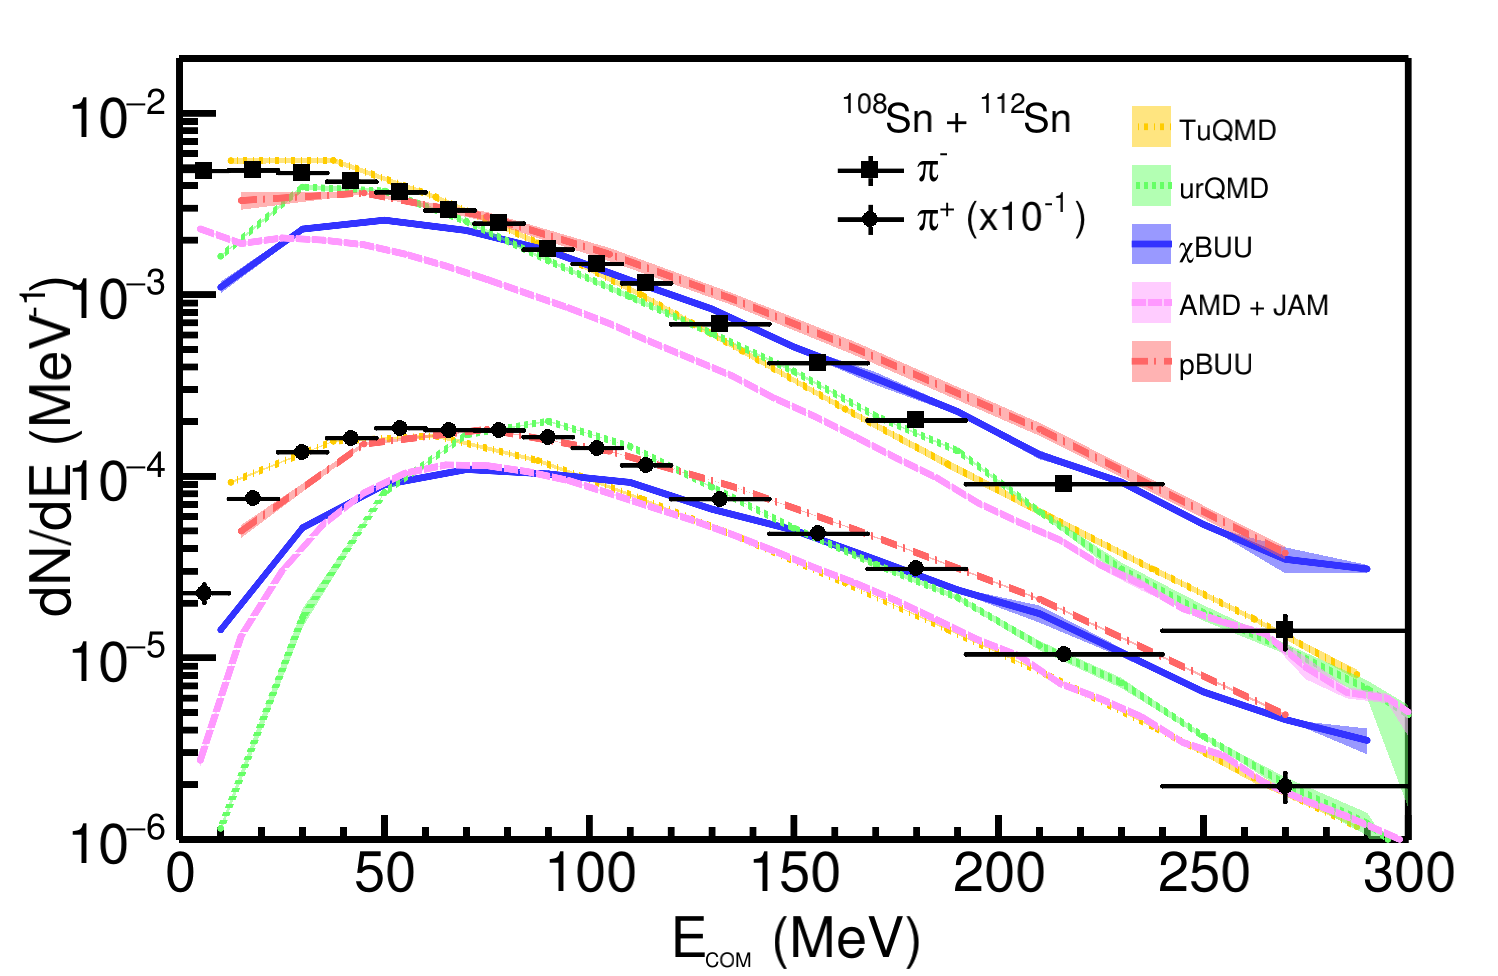
\includegraphics[width=\textwidth]{pionSpectra.png}
\caption{Pion spectra. }
\label{fig:pionspectra}
\end{figure}


%Add figure on Glauber model 
%Add figure on comparison to FOPI data

\section{Pion Yield}


\begin{table*}\centering
\ra{1.3}
\begin{tabular}{@{}cccc@{}}\toprule
System & $\pi^-$ & $\pi^+$ & $Y(\pi^-)/Y(\pi^+)$  \\
\midrule
$\tin{132}{124}$ & 0.717(24)(4) & 0.148(5)(2) & 4.84(10)(6)  \\
$\tin{108}{112}$ & 0.399(14)(3) & 0.200(8)(2) & 1.99(4)(3)  \\
%$\tin{132}{124}$ & \numerr{0.717}{0.024}{0.004} & \numerr{0.148}{0.005}{0.002} & \numerr{4.84}{0.10}{0.06}  \\
%$\tin{108}{112}$ & \numerr{0.399}{0.014}{0.003} & \numerr{0.200}{0.008}{0.002} & \numerr{1.99}{0.04}{0.03}  \\
\bottomrule
\end{tabular}
\caption{Total pion yield.}
\label{tb:pionyield}
\end{table*}







\section{$\pi^-$/$\pi^+$ Ratio}

\begin{figure}
\centering
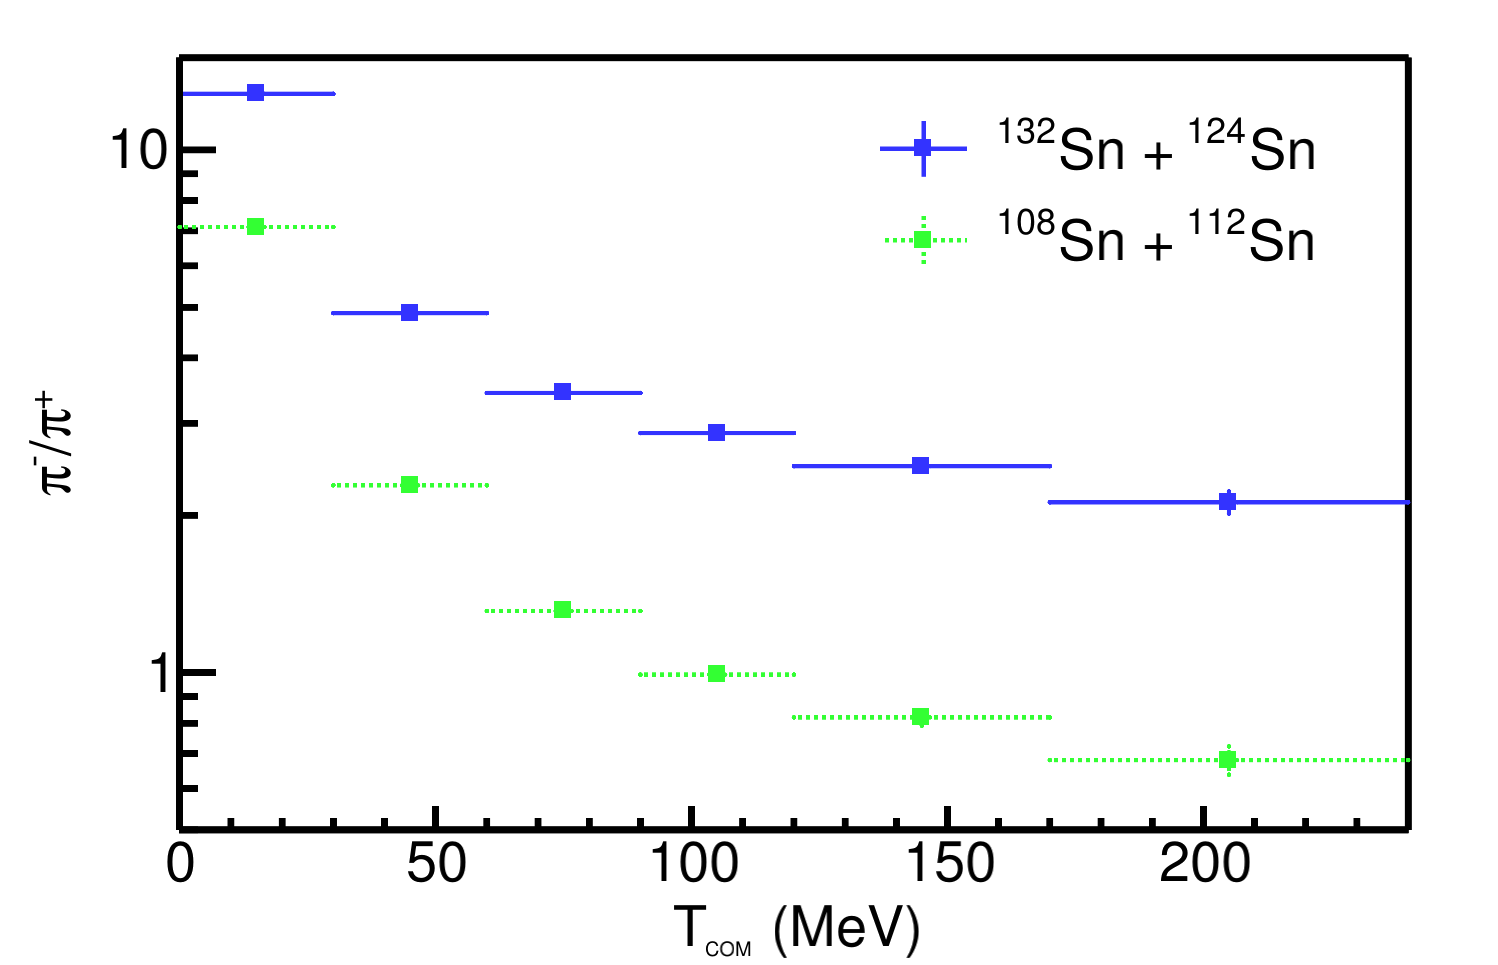
\includegraphics[width=\textwidth]{singleRatio.png}
\caption{Single ratio spectra}
\label{fig:SRspectra}
\end{figure}

%Add figure of Theory for pion ratios

\section{Pion Double Ratio}
%Add figure of Theory for pion ratios

\begin{figure}[!htb]
\centering
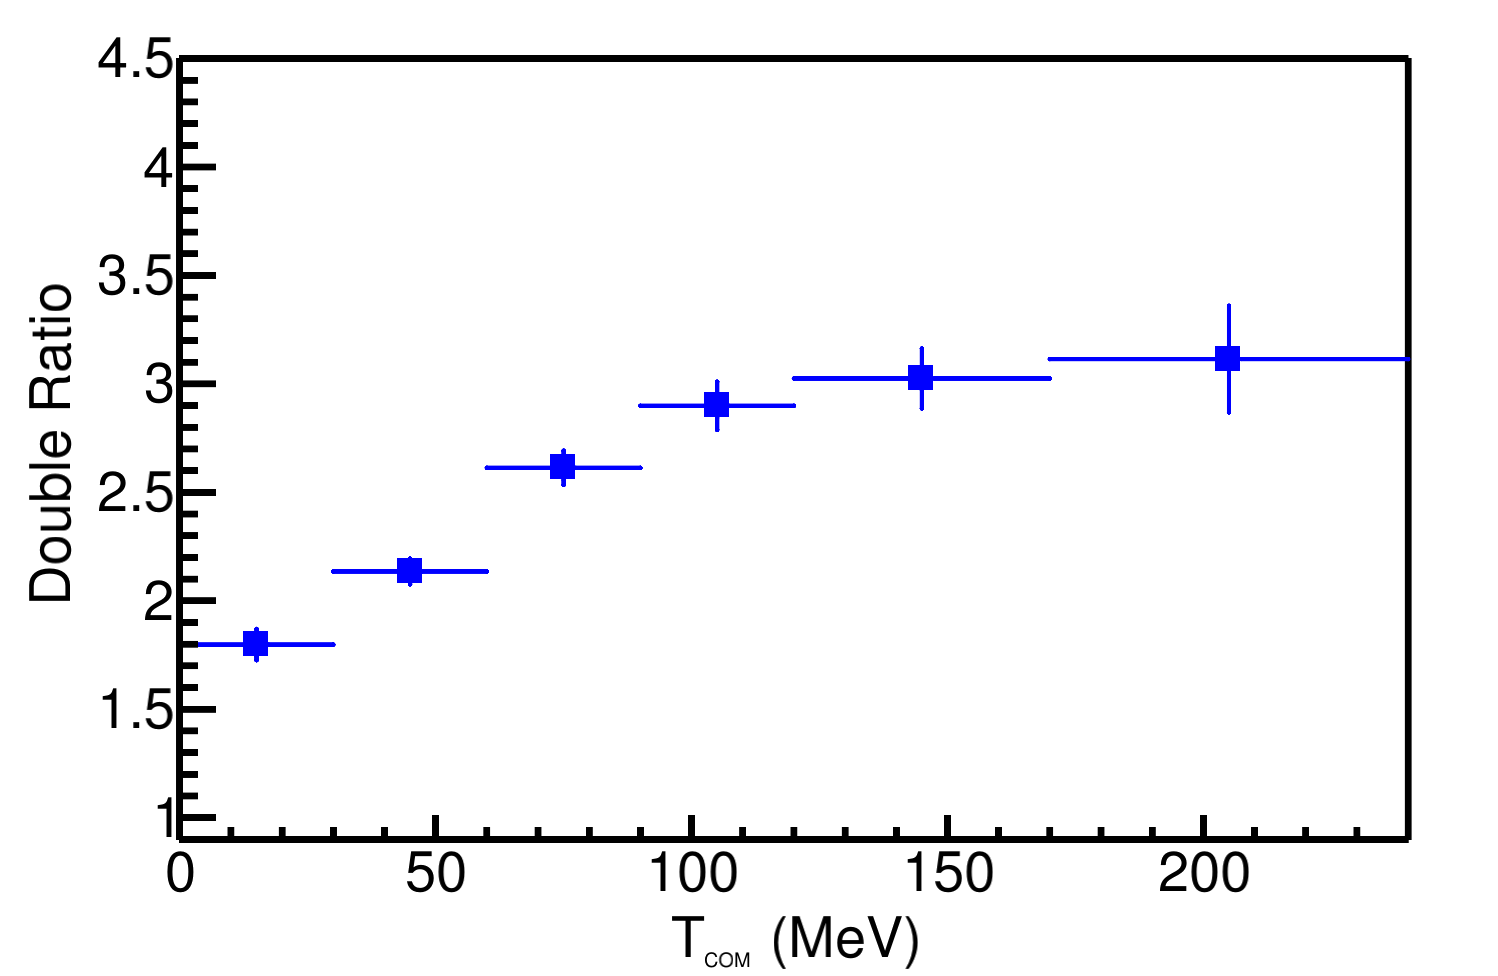
\includegraphics[width=\textwidth]{doubleRatio.png}
\caption{}
\label{fig:spectraDR}
\end{figure}




\section{Comparison to Previous Data Sets (FOPI)}
asdfasdfasd
\section{Comparison to Theory}
%Add figure of Pion spectra for different theory 
%Reference paper for multiple theories
asdfasdf

\section{Systematic Errors and Cut Variations}
\label{sec:cutvar}
dfsadfsaf
\section{Constraint on the Symmetry Energy}
%maybe not...